\chapter{Experimentación}

\section {Casos de prueba}
A continuación se describe la metodología utilizada para la evaluación experimental de las diferentes variaciones de los algoritmos de exploración. Las pruebas se realizaron de forma automatizada con el simulador Sphinx para drones de la marca Parrot. La flota consta de dos drones.

En total se cuenta con tres estrategias de exploración diferentes a evaluar. Como ya se discutió en otras secciones los algoritmos greedy son los de mayor prevalencia para resolver problemas de múltiples agentes ya que no requieren grandes capacidades computacionales y han demostrado en muchos experimentos que tienen desempeños iguales o mejores a otros tipos de algoritmos en teoría más complejos. De esta forma se optó por evaluar el algoritmo greedy contra el algoritmo basado en distribución de zonas para determinar si los algoritmos greedy resultan convenientes para resolver este problema en particular. La tercera estrategia a evaluar es un algoritmo de funcionamiento aleatorio, es decir, un algoritmo que define todos los movimientos del dron de forma aleatoria. Este algoritmo aleatorio sirve como prueba de control y los otros algoritmos deberían tener mejores rendimientos que el suyo para poder considerarse viables.

Para cada uno de los algoritmos se relevaron varias medidas. Los algoritmos cuentan con dos objetivos principales: en primer lugar deben cubrir toda la zona a explorar de la forma más homogénea y rápida posible y luego deben atender los puntos de interés con la menor demora posible. Esto lleva a que los datos relevados también se separen en dos categorías, cada una corresponde a uno de estos objetivos.
Para medir el cubrimiento del mapa se releva el porcentaje del área que fue explorada en función del tiempo, tomándose una medición cada 10 segundos y además se registra la cantidad de veces que los drones pasaron por cada ubicación del área.
Para medir el nivel de atención de los puntos de interés se releva la cantidad de veces que se desencadenó una interrupción para atender un punto de interés, si esa interrupción es de tipo normal o crítica, la cantidad de interrupciones que los drones efectivamente atendieron y cuanto tiempo demoraron en atenderla. Para cada de uno de estos registros también se releva cual fue el punto de interés al que corresponde.

El siguiente paso fue el de crear instancias de prueba sobre los que ejecutar los algoritmos. Para esto se optó por crear escenarios que sean realistas y que representen realidades diferentes, de esta forma se puede evaluar el desempeño de los algoritmos en situaciones variadas. Se diseñaron tres escenarios de diferente tamaño y con obstáculos de diferente tipo y distribución, luego para cada escenario se crearon diez instancias con variaciones aleatorias, esto permite evaluar los escenarios con menor sesgo. Las instancias difieren entre sí en la ubicación de sus puntos de interés y en el tiempo que deben ser atendidos. De esta forma podemos evaluar si existen puntos en cada escenario que resulten más difíciles de controlar. En total, cada algoritmo fue evaluado cuatro veces en cada instancia de cada escenario.
El primer escenario consiste en un galpón de aproximadamente 5000 m2. En este escenario los principales obstáculos vienen dados por paredes y racks que también forman estructuras en forma de pared. El galpón tiene una única entrada que representa un punto de interés a vigilar. Su ubicación y la frecuencia con la que debe ser atendido varía en cada instancia del escenario.

\begin{figure}[h!]
	\label{fig:comp}
	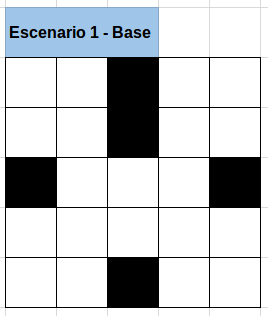
\includegraphics[width=.8\textwidth]{imagenes/chap6/image1}
	\caption{Versión base del escenario 1.}
\end{figure}

El segundo escenario consiste de un establecimiento que ocupe una cuadra entera (aproximadamente 10000 m2) compuesto por tres edificios principales y el resto del mapa es una zona de patio despejada. Los edificios definen zonas prohibidas en las que los drones no pueden entrar. En este escenario se cuenta con tres puntos de interés que representan diferentes zonas de ingreso al predio.


\begin{figure}[h!]
	\label{fig:comp}
	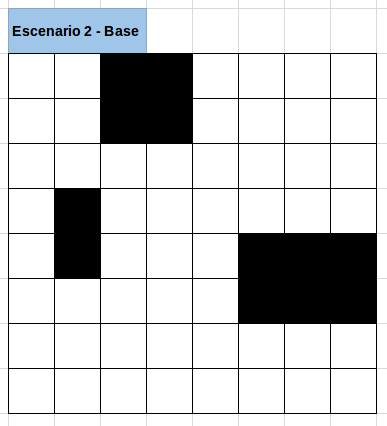
\includegraphics[width=.8\textwidth]{imagenes/chap6/image2}
	\caption{Versión base del escenario 2.}
\end{figure}

El último escenario consiste en un campo de 2 hectáreas (aproximadamente 20000 m2) en el cual hay solo algunos obstáculos aislados en forma de árboles y casas. En este caso se cuenta con cinco puntos de interés que representan corrales, puntos de entrada o la casa del dueño.


\begin{figure}[h!]
	\label{fig:comp}
	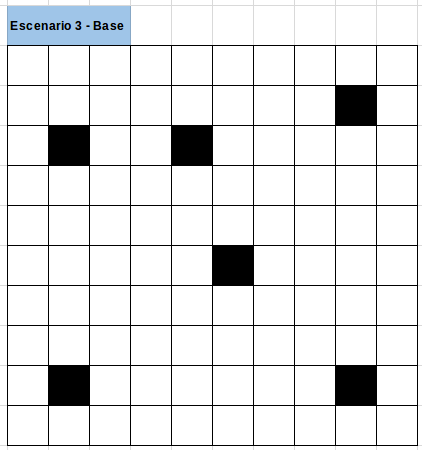
\includegraphics[width=.8\textwidth]{imagenes/chap6/image3}
	\caption{Versión base del escenario 3.}
\end{figure}

Por último se establecieron algunos datos paramétricos de interés.
La altura de vuelo se definió en 10 metros ya que a esta altura se pueden esquivar la mayoría de los obstáculos (solo hay que preocuparse por obstáculos mayores y estáticos como paredes, árboles o edificios) pero a su vez es lo suficientemente cercano al suelo para no perder calidad de imagen de la cámara, de esta forma se puede vigilar la zona de forma efectiva.
Para los drones Bebop 2 una altura de vuelo de 10 metros implica que se tiene un área de visión de 10x18 metros con la cámara apuntando directamente hacia abajo. Esto permite definir la unidad con la que se divide la matriz del área a explorar como un rectángulo de 10x18 metros. De esta forma el escenario 1 queda representado como una matriz de 5x5 unidades, el escenario 2 se representa como uno de 8x8 unidades y el escenario 3 se representa como uno de 10x10 unidades.
Se estableció un tiempo de misión de 20 minutos ya que este es un tiempo un poco menor a los 25 minutos de duración de la batería. Esto permite obtener mediciones de cuanto se puede explorar con una carga de batería dejando un colchón de 5 minutos para imprevistos.
Todos los drones despegan desde la misma ubicación, la cual representa la base a la que tienen que retornar cuando acabe la misión o en caso de emergencia.

A continuación se presenta un resumen de las características mencionadas de la evaluación experimental:


Algoritmos evaluados
Aleatorio
Este algoritmo determina los movimientos del dron de forma completamente aleatoria. Sirve principalmente como prueba de control.
Greedy basado en timestamps
Un algoritmo greedy que determina el siguiente movimiento del dron en base al tiempo que pasó desde la última vez que un dron visitó los puntos adyacentes a la posición actual en el mapa.
No greedy basado en timestamps
Un algoritmo que divide el mapa en regiones. Un dron explora una misma región hasta que esta se encuentre mayormente explorada o hasta que se detecta que hay otras por las que la flota no pasa desde hace mucho tiempo. Luego cambia de región y repite el proceso.
Tabla 2: Algoritmos evaluados























Escenario 1
Descripción
Un galpón o establecimiento de tamaño intermedio
Dimensiones físicas
5000 m2
Representación
Matriz de 5x5 unidades
Puntos de interés
1
Obstáculos
En forma de paredes
Escenario 2
Descripción
Un establecimiento de tamaño mayor que ocupe una cuadra entera
Dimensiones físicas
10000  m2
Representación
Matriz de 8x8 unidades
Puntos de interés
3
Obstáculos
En forma de zonas prohibidas
Escenario 3
Descripción
Un terreno o campo de 2 hectáreas
Dimensiones físicas
20000  m2
Representación
Matriz de 10x10 unidades
Puntos de interés
5
Obstáculos
En forma de puntos aislados
Tabla 3: Descripción de escenarios


Instancias
Instancias por escenario
10
Cantidad de ejecuciones por instancia y por algoritmo
4
Posición de los POI
Aleatoria
Frecuencia de atención de los POI
Aleatoria
Tabla 4: Descripción de instancias


Datos paramétricos
Cantidad de drones
2
Altura de vuelo
10 metros
Tamaño de la unidad de vuelo
10x18 metros
Tiempo de misión
20 minutos
Zona de despegue
Una única base en la posición (0,0) de cada mapa
Tabla 5: Datos paramétricos

Especificaciones técnicas
Tiempo total de simulación
120 horas
Sistema operativo
Ubuntu 16.04 64 bits
Procesador
Intel® Core™ i7-4510U CPU @ 2.00GHz × 4
Memoria RAM
8GB
Tarjeta gráfica
Intel® Haswell Mobile
Simulador
Sphinx 0.29.1, Gazebo 7.0.1
Tabla 6: Especificaciones técnicas

Resultados
FALTA ANALIZAR RESULTADOS

